\chapter{Progettazione e codifica}
\label{cap:progettazione-codifica}

\emph{In questo capitolo si descrive la progettazione e la codifica del sistema. Si inizia con una panoramica generale del sistema, per poi passare a una descrizione dettagliata delle varie componenti.}

\section{Architettura ad alto livello}
Le fasi di un flusso di lavoro per l'\gls{idpg} possono variare in base al caso d'uso specifico e ai requisiti aziendali, ma esistono alcune fasi comuni che sono generalmente presenti in qualsiasi processo \gls{idpg}. Tali flussi di lavoro trovano applicazione in diversi ambiti, come l'elaborazione di moduli fiscali, reclami, note mediche, moduli di nuovi clienti, fatture, contratti legali, e molti altri documenti aziendali. 

Nel contesto del presente progetto, l'obiettivo è stato quello di rispondere alla richiesta dell'azienda ospitante di automatizzare la catalogazione e l'elaborazione delle email e dei relativi documenti allegati. A tal fine, è stato progettato un flusso di lavoro articolato in diverse fasi, ciascuna delle quali contribuisce a trasformare i documenti non strutturati in informazioni strutturate e utilizzabili. Le fasi individuate per il processo di elaborazione dei documenti dalle email sono le seguenti:

\begin{itemize}
  \item \textbf{\emph{Data Capture}}: Questa fase riguarda l'estrazione degli allegati dalle email. I file vengono archiviati e aggregati in modo sicuro, garantendo la corretta gestione dei dati fin dal primo momento. Questo passaggio è cruciale per assicurare che tutte le informazioni necessarie siano raccolte e pronte per le fasi successive del processo.
  
  \item \textbf{\emph{Classification}}: Una volta acquisiti, i documenti vengono classificati in base al loro contenuto. Questa fase consiste nell'assegnazione di ciascun documento a una specifica pipeline di elaborazione, in base alla tipologia di documento identificata. La corretta classificazione è fondamentale per assicurare che ogni documento segua il percorso di elaborazione più appropriato.

  \item \textbf{\emph{Extraction}}: Durante questa fase, vengono estratte le informazioni aziendali rilevanti dai documenti. Si tratta di un processo automatizzato in cui i dati chiave vengono isolati e resi disponibili per ulteriori analisi. L'accuratezza di questa fase è determinante per il successo complessivo del flusso di lavoro, poiché influisce direttamente sulla qualità delle informazioni che verranno utilizzate.

  \item \textbf{\emph{Validation}}: Una volta estratte, le informazioni devono essere validate. In questa fase, vengono applicate regole di business per assicurare che i dati siano corretti e completi. Inoltre viene controllata la confidenza per ogni informazione estratta, riducendo il margine di errore e assicurando l'affidabilità del processo.

  \item \textbf{\emph{Storage}}: Infine, le informazioni validate vengono salvate in un database aziendale. Questo passaggio è essenziale per garantire che i dati estratti siano facilmente accessibili per future consultazioni o analisi, completando così il ciclo di trasformazione dei documenti.
\end{itemize}

Questo flusso di lavoro, progettato per ottimizzare l'elaborazione automatizzata dei documenti, rappresenta un passo significativo verso l'efficienza operativa e la riduzione dei costi aziendali. Tale flusso è stato implementato utilizzando i servizi di \gls{awsg}, in particolare \emph{AWS Lambda}, \emph{Amazon Textract}, \emph{Amazon Comprehend} e \emph{Amazon DynamoDB}. Attraverso \emph{AWS Step Functions} è stato possibile orchestrare in modo efficiente le diverse fasi del processo, garantendo una gestione ottimale dei dati e una maggiore scalabilità.\\
L'architettura proposta (figura \ref{fig:architettura-alto-livello}) è stata concepita all'interno del cloud AWS affidato da \myCompany, in particolare nel portale denominato \emph{WikiAi}. Le risorse principali sono state concepite nella regione Francoforte (eu-central-1) e sono state organizzate in base alle esigenze del progetto. \\
Come precedentemente menzionato l'architettura comprende diverse fasi, ognuna delle quali svolge un ruolo specifico nel processo di elaborazione dei documenti. In particolare, il flusso di lavoro è stato progettato per classificare gli allegati delle email in quattro categorie principali: ordini, fatture, contratti e non classificato. Inoltre, il sistema è progettato per estrarre informazioni specifiche dai documenti appartenenti alle prime tre categorie, escludendo la categoria non classificato.

% Inserisci l'immagine che occupa l'intera pagina
\begin{figure}[p]
    \centering
    \begin{turn}{-90}
      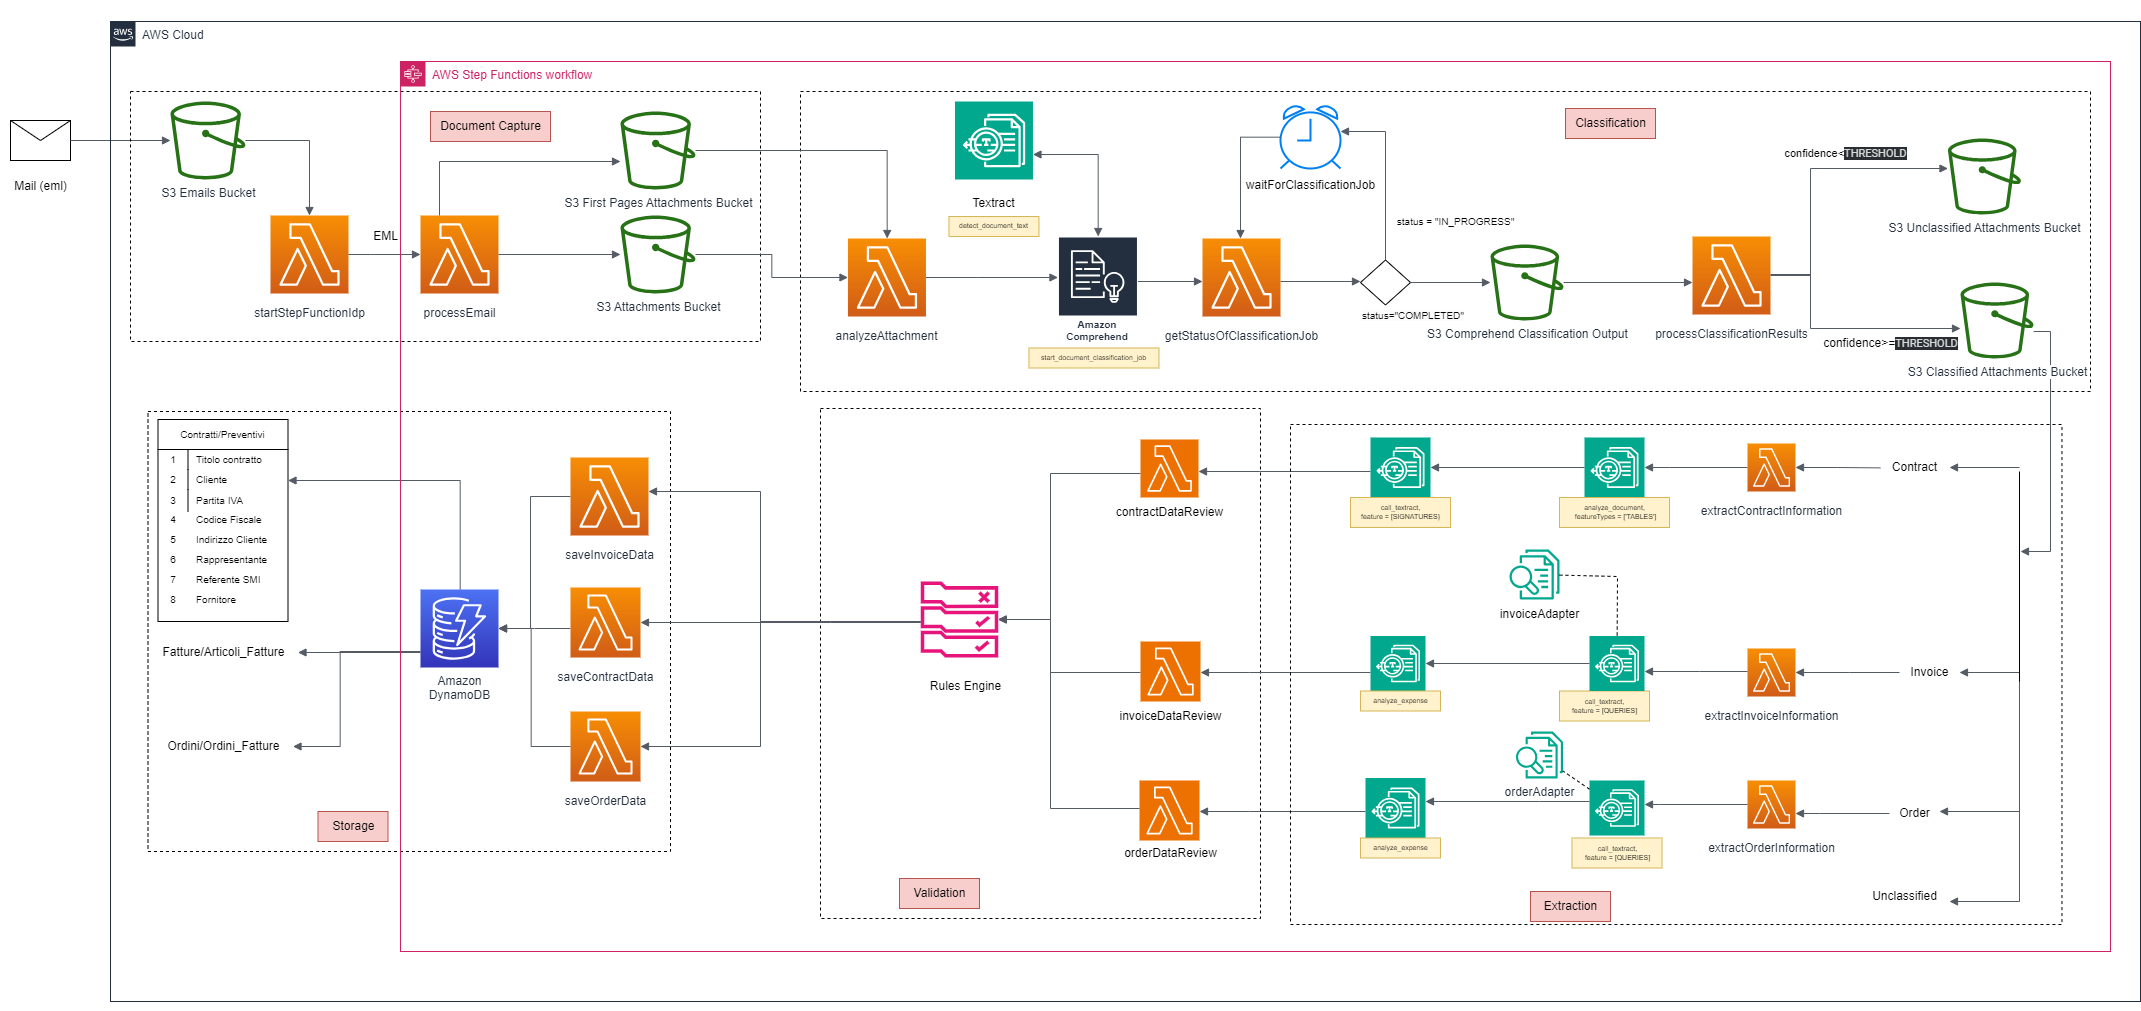
\includegraphics[width=\textheight]{img/design/classificatore_email.drawio.png}
    \end{turn}
    \captionof{figure}{Architettura ad alto livello del sistema}
    \label{fig:architettura-alto-livello}
\end{figure}

Come precedentemente menzionato, gran parte del flusso di lavoro è stato orchestrato tramite AWS Step Functions (nella figura \ref{fig:architettura-alto-livello} è evidenziato tramite un riquadro in rosso) e in particolare tramite la state machine denominata \emph{IdpStateMachine}. La figura \ref{fig:IDP_state_machine}, creata tramite l'editor di AWS, mostra la struttura della state machine e le diverse fasi coinvolte nel processo di elaborazione dei documenti.   
\begin{figure}[p]
    \centering
    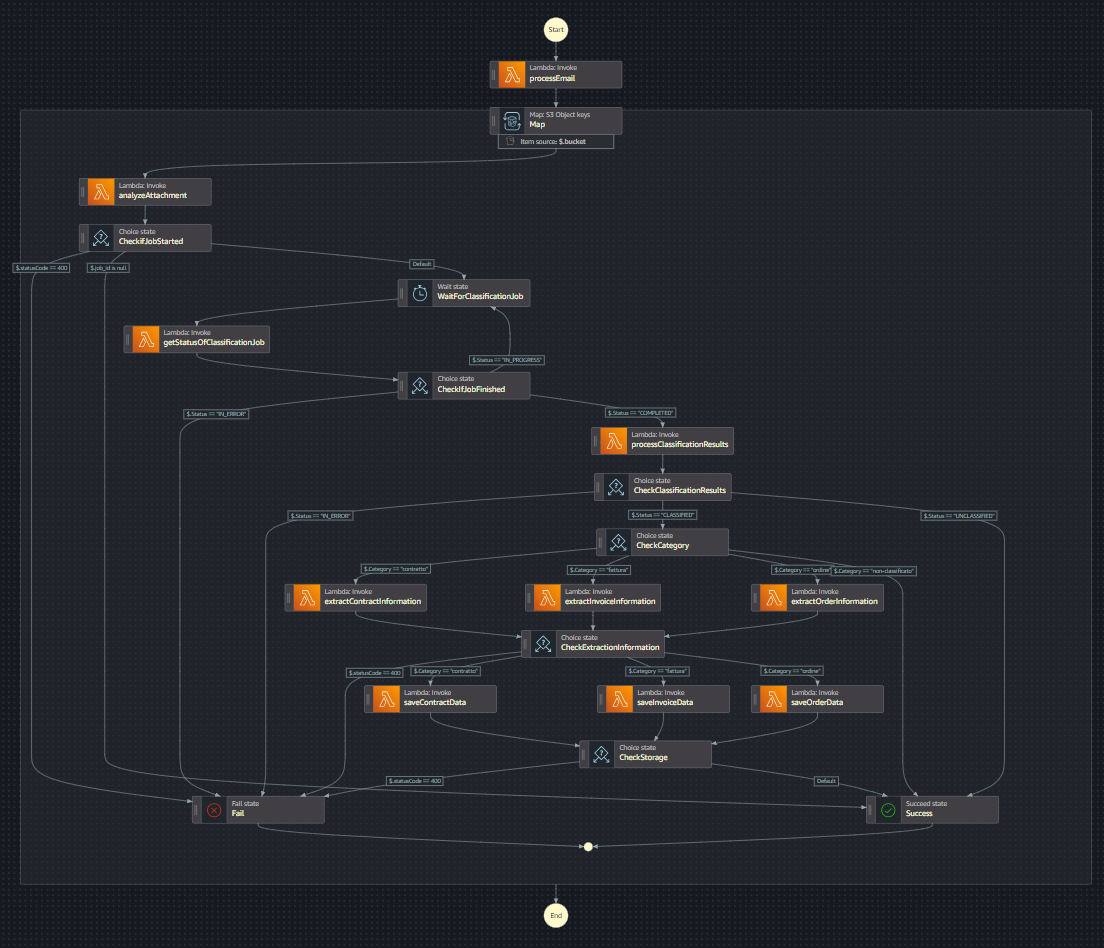
\includegraphics[width=1.1\textwidth, height=0.9\textheight]{img/design/IdpStateMachine.png}
    \caption{State machine "IdpStateMachine" di AWS Step Functions}
    \label{fig:IDP_state_machine}
\end{figure}
\section{Risorse e servizi AWS utilizzati}
\label{sec:risorse-servizi-aws}
Il sistema è stato progettato utilizzando una serie di risorse e servizi AWS, ciascuno dei quali svolge un ruolo specifico nel processo di elaborazione dei documenti. Le principali risorse e servizi utilizzati includono:
\begin{itemize}
    \item Amazon S3
    \begin{itemize}
        \item \emph{S3 Emails Bucket}: contenente le email in formato \texttt{.eml}.
        \item \emph{S3 Attachments Bucket}: contenente gli allegati estratti dalle email.
        \item \emph{S3 First Pages Attachments Bucket}: contenente le prime pagine dei file PDF estratte dagli allegati.
        \item \emph{S3 Comprehend Classification Output}: contenente i risultati della classificazione di Comprehend.
        \item \emph{S3 Classified Attachments Bucket}: contenente gli allegati classificati.
        \item \emph{S3 Unclassified Attachments Bucket}: contenente gli allegati non classificati.
    \end{itemize}
    \item AWS Lambda
    \begin{itemize}
        \item \emph{startStepFunctionIdp}: attiva l'esecuzione della state machine IdpStateMachine.
        \item \emph{processEmail}: estrae gli allegati dalle email.
        \item \emph{analyzeAttachment}: utilizza il classificatore di Comprehend per classificare gli allegati.
        \item \emph{getStatusOfClassificationJob}: controlla lo stato del job di classificazione.
        \item \emph{processClassificationResults}: elabora l'output della classificazione di Comprehend.
        \item \emph{extractContractInformation}: estrae le informazioni dai contratti.
        \item \emph{extractInvoiceInformation}: estrae le informazioni dalle fatture.
        \item \emph{extractOrderInformation}: estrae le informazioni dagli ordini.
        \item \emph{contractDataReview}: permette la revisione manuale delle informazioni estratte dai contratti.
        \item \emph{invoiceDataReview}: permette la revisione manuale delle informazioni estratte dalle fatture.
        \item \emph{orderDataReview}: permette la revisione manuale delle informazioni estratte dagli ordini.
        \item \emph{saveContractInformation}: salva le informazioni estratte dai contratti in DynamoDB.
        \item \emph{saveInvoiceInformation}: salva le informazioni estratte dalle fatture in DynamoDB.
        \item \emph{saveOrderInformation}: salva le informazioni estratte dagli ordini in DynamoDB.
    \end{itemize}
    \item AWS Step Functions
    \begin{itemize}
        \item \emph{IdpStateMachine}: gestisce il flusso di lavoro.
    \end{itemize}
    \item Amazon Comprehend
    \begin{itemize}
        \item \emph{document-classifier}: modello personalizzato per la classificazione degli allegati.
        \item \emph{custom-document-classifier-flywheel}: flywheel per la creazione di modelli personalizzati che riporta tre differenti \gls{datasetg}:
        \begin{itemize}
            \item \emph{document-classifier-train}: \gls{datasetg} di training per la prima versione del modello.
            \item \emph{trainingFatture}: \gls{datasetg} di training per la seconda versione del modello.
            \item \emph{my-training-set}: \gls{datasetg} di training per la seconda versione del modello.
        \end{itemize}
    \end{itemize}
    \item Amazon Textract
    \begin{itemize}
        \item \emph{analyze\_document}: estrae le informazioni principali dai documenti.
        \item \emph{call\_textract}: funzione simile a \emph{analyze\_document} ma con funzionalità aggiuntive.
        \item \emph{adapter checksInvoiceAdapter}: adattatore utilizzato per le custom queries per l'estrazione delle informazioni dalle fatture.
        \item \emph{adapter checksOrderAdapter}: adattatore utilizzato per le custom queries per l'estrazione delle informazioni dagli ordini.
    \end{itemize}
    \item Amazon DynamoDB
    \begin{itemize}
        \item \emph{Contratti}: tabella contenente le informazioni estratte dai contratti.
        \item \emph{Preventivi}: tabella contenente le informazioni estratte dai preventivi.
        \item \emph{Fatture}: tabella contenente le informazioni estratte dalle fatture.
        \item \emph{Articoli\_Fatture}: tabella contenente le informazioni relative agli articoli delle fatture.
        \item \emph{Ordini}: tabella contenente le informazioni estratte dagli ordini.
        \item \emph{Articoli\_Ordini}: tabella contenente le informazioni relative agli articoli degli ordini.
    \end{itemize}
\end{itemize}
\section{Estrazione degli allegati}
\label{sec:estrazione-allegati}
Inizialmente, l'indicazione fornita dall'azienda richiedeva un'analisi del contenuto delle email, seguita da una classificazione basata sull'elaborazione del linguaggio naturale e sui metadati contenuti. Tuttavia, con il chiarimento delle categorie di interesse (ordini, fatture e contratti), ho deciso di concentrare l'attenzione sull'estrazione degli allegati presenti nelle email piuttosto che sul contenuto testuale delle stesse.

Questa scelta è giustificata dal fatto che i documenti di interesse per l'azienda sono spesso inclusi come allegati nelle email, rendendo l'estrazione degli allegati un approccio più diretto ed efficace. Inoltre, il contenuto delle email è spesso irrilevante o solo parzialmente utile per il processo di classificazione.

L'obiettivo principale di questa fase è quindi quello di ricavare gli allegati dalle email per poterli successivamente classificare e analizzare. Il processo è strutturato nelle seguenti fasi:

\begin{itemize}
    \item \textbf{Caricamento del file \texttt{.eml}}: Il processo inizia con il caricamento del file \texttt{.eml} nel bucket "S3 Emails Bucket", che funge da archivio per le email da analizzare.
    
    \item \textbf{Attivazione della funzione Lambda "StartStepFunctionIdp"}: L'inserimento del file \texttt{.eml} nel bucket attiva la funzione Lambda \emph{StartStepFunctionIdp}, la quale avvia l'esecuzione della state machine \emph{IdpStateMachine} di AWS \emph{Step Functions}. Questa state machine gestisce l'intero flusso di lavoro automatizzato.

    \item \textbf{Estrazione degli allegati}: La state machine avvia la funzione Lambda \emph{processEmail}, responsabile dell'estrazione degli allegati dalle email. Questa funzione è essenziale per isolare i documenti di interesse dal file \texttt{.eml}.
    \item \textbf{Caricamento degli allegati}: Una volta estratti, gli allegati vengono caricati nel bucket \emph{S3 Attachments Bucket}. Gli allegati, che possono essere in vari formati (PDF, PNG, JPG, TXT, DOC, DOCX, ecc.), vengono archiviati in una cartella il cui nome corrisponde a quello della mail da cui provengono (file \texttt{.eml}). In aggiunta, le prime pagine dei file PDF vengono salvate nel bucket \emph{S3 First Pages Attachments Bucket} e vengono archiviati nello stesso modo. 
\end{itemize}
Gli allegati, ora presenti nei bucket \emph{S3 Attachments Bucket} e \emph{S3 First Pages Attachments Bucket}, sono pronti per essere classificati e analizzati nelle fasi successive del processo. 
\section{Classificazione dei documenti}
\label{sec:classificazione-documenti}
Inizialmente, si era presa in considerazione l'idea di classificare le email in base al loro contenuto utilizzando modelli di \gls{machinelearningg} offerti da \emph{Amazon SageMaker}. Tuttavia, con il chiarimento delle categorie di interesse durante lo stage (ordini, fatture e contratti), si è deciso di focalizzarsi sull'estrazione e la classificazione degli allegati presenti nelle email, piuttosto che sul contenuto testuale delle stesse. Questo approccio ha semplificato significativamente il processo di classificazione, poiché i metadati (denominati anche \textit{features} nel contesto del \gls{machinelearningg}) si riducono al semplice testo estratto dagli allegati e tale caso d'uso si presta bene all'utilizzo di \emph{Amazon Comprehend} per la classificazione ed in particolare per la creazione di un modello personalizzato.\\
Sebbene in una fase iniziale fosse stato considerato e provato l'uso del servizio \emph{Amazon Bedrock} per classificare i documenti, in particolare con il modello \emph{Claude-3}, questa opzione è stata successivamente scartata a favore di un modello personalizzato, ritenuto più adatto alle specifiche esigenze del progetto e meno costoso.\\
In questo contesto, l'utilizzo di \emph{Amazon Textract} e \emph{Amazon Comprehend} si è rivelato cruciale per l'accuratezza della classificazione.\\
La fase di classificazione degli allegati (figura \ref{fig:architettura-alto-livello} riquadro denominato \emph{Classification}) si articola nelle seguenti operazioni:

\begin{itemize}
    \item \textbf{Caricamento del file \texttt{.eml} e attivazione della pipeline}: Dopo l'estrazione degli allegati dalle email, descritta nella Sezione \ref{sec:estrazione-allegati}, i documenti vengono preparati per la classificazione. La funzione Lambda \emph{analyzeAttachment} utilizza il classificatore di Amazon Comprehend denominato 
    \emph{document-classifier} per analizzare la prima pagina degli allegati ricavandole dal bucket \emph{S3 First Pages Attachments Bucket}. Il testo viene estratto tramite la funzione \texttt{detect\_document\_text} di \emph{Amazon Textract}, che converte i contenuti dei documenti in un formato testuale adatto per l'analisi.

    \item \textbf{Salvataggio del risultato della classificazione}: I risultati del job di classificazione, composti da un file JSON che riporta la categoria assegnata e il relativo livello di confidenza, vengono salvati nel bucket \emph{S3 Comprehend Classification Output}. Questo passaggio consente di archiviare in modo strutturato i risultati che saranno successivamente elaborati per l'estrazione delle informazioni.

    \item \textbf{Processamento dei risultati della classificazione}: Al termine del job di classificazione, la funzione Lambda \emph{processClassificationResults} viene attivata per salvare gli allegati classificati nei \emph{bucket} appropriati. Infatti se la confidenza del modello è superiore a una soglia (\textit{threshold}) predefinita, l'allegato viene salvato nel \emph{bucket} \emph{S3 Classified Attachments Bucket}; altrimenti, viene salvato nel \emph{bucket} \emph{S3 Unclassified Attachments Bucket}. Gli allegati sono archiviati in cartelle che riportano la categoria di classificazione (ordine, fattura, contratto, non classificato). Questa organizzazione è fondamentale per facilitare la gestione e l'analisi successiva degli allegati, compresi quelli non classificati, che possono essere esaminati in dettaglio in un secondo momento.
\end{itemize}

Una precisazione importante riguarda la distinzione tra gli allegati salvati nel bucket \emph{S3 Classified Attachments Bucket} e quelli salvati nel bucket \emph{S3 Unclassified Attachments Bucket} 
all'interno della cartella "non classificato". Gli allegati presenti nel bucket \emph{S3 Unclassified Attachments Bucket} sono quelli per cui il livello di confidenza del modello è inferiore alla soglia predefinita. Al contrario, gli allegati presenti nella cartella "non classificato" del \emph{S3 Classified Attachments Bucket} sono stati classificati con una confidenza superiore alla soglia, ma la categoria assegnata è comunque "non classificato", indicando la classificazione sia stata effettuata con un certo grado di sicurezza.
\subsection{Creazione del modello di classificazione personalizzato}
\label{subsec:training-modello}
La creazione di un modello di classificazione personalizzato con Amazon Comprehend richiede la disponibilità di un \gls{datasetg} ampio, significativo e bilanciato, capace di distinguere con precisione le categorie di interesse. È fondamentale che il \gls{datasetg} sia etichettato correttamente, in modo che ogni documento sia associato alla giusta categoria di appartenenza.

Durante la fase di etichettatura, sono emerse alcune considerazioni chiave. I documenti da analizzare sono prevalentemente file PDF, spesso costituiti da scansioni. Per garantire coerenza nel processo di training, si è deciso di utilizzare esclusivamente documenti in formato PDF. Inoltre, è stato scelto di utilizzare unicamente le prime pagine di tali documenti per il training del modello. Questa scelta è stata motivata dal fatto che le prime pagine contengono generalmente le informazioni più rilevanti per la classificazione. Inoltre, considerando che il costo dell'analisi è proporzionale al numero di pagine, la riduzione del numero di pagine ha comportato una significativa riduzione dei costi operativi, soprattutto in documenti che possono arrivare fino a 30 o più pagine.

Tuttavia, queste scelte hanno anche portato a una riduzione della varietà dei dati utilizzati per il training, il che potrebbe potenzialmente introdurre \glsfirstoccur{\gls{biasg}} nel modello, limitando la sua capacità di generalizzare su nuovi dati. \\
Del modello personalizzato denominato \emph{document-classifier} sono state create due versioni, ciascuna addestrata su dei \gls{datasetg} specifici. 
Per la prima versione del modello, denominata \emph{document-classifier-version-1}, sono stati utilizzati 47 documenti etichettati.\\
Per la seconda versione del modello, denominata \emph{Comprehend-Generated-v1-
461f932}, generata tramite il processo di \gls{activelearningg} con \emph{Flywheel}, sono stati utilizzati dei \gls{datasetg} di training di 56 documenti che si vanno ad aggiungere ai 47 documenti utilizzati per la versione precedente.
Per creare e distribuire il modello personalizzato, sono state seguite le seguenti fasi: \emph{Analisi del dataset}, \emph{Preprocessing}, \emph{Training}, \emph{Valutazione} e \emph{Test del modello}.
\paragraph*{Analisi del dataset}
L'\emph{analisi del dataset} è fondamentale per comprendere la distribuzione delle categorie e valutare l'adeguatezza dei dati per la successiva fase di addestramento. Per i \gls{datasetg} utilizzati nelle varie iterazioni, le percentuali di distribuzione delle categorie (ordini, fatture, contratti e non classificato) sono state attentamente monitorate per garantire un bilanciamento adeguato.\\
Per il primo dataset di training, denominato \emph{document-classifier-train}, sono stati utilizzati 47 documenti etichettati, distribuiti nel modo seguente:
\begin{itemize}
    \item 25 contratti (53.19\%)
    \item 3 fatture (6.38\%)
    \item 5 ordini (10.64\%)
    \item 14 non classificati (29.79\%)
\end{itemize}
Per il secondo dataset di training, denominato \emph{trainingFatture}, sono stati utilizzati 26 documenti etichettati, distribuiti nel modo seguente:
\begin{itemize}
    \item 1 ordine (3.85\%)
    \item 25 fatture (96.15\%)
\end{itemize}
Per il terzo dataset di training, denominato \emph{my-training-set}, sono stati utilizzati 30 documenti etichettati, distribuiti nel modo seguente:
\begin{itemize}
    \item 10 fatture (33.33\%)
    \item 10 non classificati (33.33\%)
    \item 10 ordini (33.33\%)
\end{itemize}
Tali scelte sono state guidate dalla necessità di garantire un bilanciamento adeguato delle categorie, in modo da evitare che il modello sia influenzato da una distribuzione sbilanciata dei dati. Inoltre, è stato fondamentale assicurare che i documenti etichettati fossero rappresentativi delle categorie di interesse, in modo da garantire che il modello fosse in grado di generalizzare su nuovi dati.

\paragraph*{Preprocessing}
Il preprocessing dei dati è una fase critica del processo di addestramento. Le operazioni principali sono state:

\begin{itemize}
    \item \textbf{Estrazione del testo tramite Amazon Textract}: Il testo contenuto nelle prime pagine dei PDF è stato estratto utilizzando \emph{Amazon Textract} tramite l'\gls{apig} \texttt{call\_textract}. 
    \item \textbf{Creazione del file CSV}: I dati estratti sono stati organizzati in un file CSV, con una colonna per la categoria di classificazione e una per il testo.
    \item \textbf{Caricamento del file CSV}: Il file di training CSV è stato caricato su \emph{Amazon S3} tramite \emph{Flywheel}, per essere utilizzato nel processo di \emph{training}.
\end{itemize}

\paragraph*{Training}
Durante la fase di {training}, il file CSV creato in precedenza è stato utilizzato per addestrare una nuova versione del classificatore personalizzato all'interno di \emph{Amazon Comprehend}. Il processo di training è stato eseguito utilizzando il servizio \emph{Flywheel}, che consente di creare e gestire modelli personalizzati in modo efficiente. Il modello è stato addestrato su un'istanza \emph{ml.m5.xlarge} per garantire prestazioni ottimali e tempi di risposta rapidi.

\paragraph*{Valutazione}
La valutazione del modello è stata condotta utilizzando metriche standard, che hanno riportato i seguenti risultati per entrambe le versioni del modello:
\begin{itemize}
    \item Precision: 1.0
    \item Recall: 1.0
    \item F1: 1.0
    \item Accuracy: 1.0
    \item Micro precision: 1.0
    \item Micro recall: 1.0
    \item Micro F1: 1.0
\end{itemize}
Questi risultati indicano una performance ottimale del modello sulle classi di interesse.\\
TO DO: spiegare meglio le metriche di valutazione.

\paragraph*{Test del modello}
Per testare il modello, è sufficiente caricare il file desiderato in un \emph{bucket S3} e avviare un \emph{job} di classificazione. Il modello restituirà la categoria di classificazione assegnata al documento e il livello di confidenza associato, permettendo così una verifica immediata delle sue prestazioni.

\subsection{Processo di Active Learning con Flywheel}
Per migliorare il modello nel tempo, è stato utilizzato il processo di \glsfirstoccur{\gls{activelearningg}} implementato tramite il servizio \emph{Flywheel} di \emph{Amazon Comprehend}. Questo approccio consente di iterare sul modello, migliorandolo progressivamente sulla base dei nuovi dati e delle prestazioni ottenute. Il processo segue questi passaggi:

\begin{itemize}
    \item \textbf{Creazione di un \emph{dataset Flywheel}}: Si parte con la definizione di un \emph{dataset} contenente i documenti etichettati, che verrà utilizzato per l'addestramento del modello.
    \item \textbf{Inizializzazione di un'iterazione \emph{Flywheel}}: Viene avviata un'iterazione di \emph{Flywheel}, durante la quale il modello viene addestrato sui dati disponibili.
    \item Attivazione del nuovo modello: Sulla base dei risultati dell'iterazione, viene deciso se attivare il nuovo modello. La decisione si basa su parametri predefiniti, come le metriche di precisione, recall e F1 score.
\end{itemize}

\section{Estrazione delle informazioni}
\label{sec:estrazione-informazioni}
In questa fase l'obiettivo è l'estrazione delle informazioni associate a ciascuna categoria escludendo la categoria non classificato. A partire dai risultati di classificazione della fase precedente si è analizzato il metodo migliore per poter estrarre le informazioni ricercate dalle categorie di contratti, ordini e fatture. Per ciascuna categoria
utilizzata una funzione \emph{lambda} che tramite \emph{Amazon Textract} estrae le informazioni
principali dai documenti. Per ciascuna delle informazioni estratte viene riportata
anche la confidenza associata utile nella fase successiva.\\
Fondamentalmente sono stati analizzati diversi metodi utilizzando differenti servizi per aderire a tale scopo:
\begin{itemize}
    \item Comprehend custom entities
    \item Amazon Bedrock con il modello Claude-3
    \item Servizi di Amazon Textract
\end{itemize}
Per ciascuna categoria è stata fatta dunque un'analisi che ha riguardato i costi oltre che l'efficacia del servizio.\\
\subsection{Estrazione delle informazioni dai contratti}
\label{subsec:estrazione-contratti}
Per l'estrazione delle informazioni dai contratti, è stata adottata una soluzione efficace e a basso costo, sfruttando la struttura uniforme di questi documenti. I contratti analizzati presentano una tabella standardizzata che contiene le seguenti informazioni chiave:

\begin{itemize}
    \item Titolo del contratto
    \item Cliente
    \item Partita IVA del cliente
    \item Codice fiscale del cliente
    \item Indirizzo del cliente
    \item Rappresentante legale del cliente
    \item Referente SMI
    \item Fornitore
\end{itemize}

La strategia implementata si basa sull'identificazione di questa tabella e sull'estrazione automatizzata dei campi utilizzando le conoscenze predefinite sulla struttura del documento. Per estrarre le informazioni desiderate, è stato impiegato \emph{Amazon Textract}, utilizzando la funzione \texttt{analyze\_document} con l'opzione \texttt{TABLES}, che consente di estrarre in modo efficiente i dati tabulari presenti nella prima pagina del contratto.

Per distinguere tra preventivi e contratti, è stata adottata una strategia basata sulla rilevazione delle firme all'interno del documento, sempre utilizzando \emph{Amazon Textract}, ma con la funzione \texttt{SIGNATURES}. Il processo prevede l'analisi delle pagine a partire dall'ultima, alla ricerca di firme. Se una firma viene rilevata, il documento viene classificato come contratto. Se, invece, al termine dell'analisi di tutte le pagine, non viene trovata alcuna firma, il documento viene classificato come preventivo.

Il risultato di questa analisi viene salvato in un file JSON di output, includendo un campo \texttt{is\_contract} che indica se il documento è stato classificato come contratto o preventivo. In caso di rilevamento di una firma, viene registrato anche il livello di confidenza associato. Se non viene trovata alcuna firma, la classificazione come preventivo viene effettuata con una confidenza del 100\%. In entrambi i casi, viene applicata una soglia (\textit{threshold}) di confidenza per garantire l'accuratezza del processo di rilevazione delle firme.

Questa soluzione permette di distinguere in modo efficace tra contratti e preventivi, sfruttando le funzionalità avanzate di \emph{Amazon Textract} e mantenendo i costi operativi contenuti, senza compromettere l'affidabilità e la precisione del processo.

\subsection{Estrazione delle informazioni dalle fatture}
\label{subsec:estrazione-fatture}
Per l'estrazione delle informazioni dalle fatture, sono state considerate diverse tecnologie, valutandone costi ed efficacia. Le soluzioni analizzate includono:

\begin{itemize}
    \item Amazon Textract, in particolare la funzione \texttt{analyze\_expense}
    \item Comprehend Custom Entity Recognition
    \item Amazon Bedrock con il modello Claude-3
    \item Utilizzo di \textit{queries} e \textit{custom queries} (adapters) di Amazon Textract
\end{itemize}

Nella tabella seguente (\ref{tab:costi-estrazione}) sono riportati i costi stimati per l'estrazione delle informazioni associate a ordini e fatture utilizzando i servizi AWS identificati. 
Il costo combinato di Amazon Textract e Claude-3 è calcolato come segue:
\begin{itemize}
  \item \$15 per 1000 pagine elaborate tramite Amazon Textract.
  \item Claude-3 ha un costo di \$0,00025 per 1000 token di input, dove un token corrisponde a circa 4 caratteri.
\end{itemize}
Il costo per utilizzare Amazon Comprehend per il riconoscimento personalizzato delle entità è calcolato come segue:
\begin{itemize}
  \item \$0,0001 per unità (100 caratteri) fino a 10 milioni di unità.
  \item Dopo 10 milioni di unità, il costo è di \$0,00005 per unità, e dopo 50 milioni di unità, il costo scende a \$0,000025 per unità.
  \item Un documento ha in media 10.000 caratteri, quindi il costo per 1000 pagine è approssimativamente \$1,00.
  \item Il costo orario per l'addestramento di un nuovo modello è di \$3, con un massimo di 10 ore, portando il totale a circa \$31.
\end{itemize}

\begin{table}[h]
  \centering
  \begin{tabular}{|c|c|}
    \hline
    \textbf{Servizio} & \textbf{Costo} \\
    \hline
    AnalyzeExpense & \$10 per 1000 pagine \\
    \hline
    Queries & \$15 per 1000 pagine \\
    \hline
    Textract + Claude-3 & \$17 per 1000 pagine \\
    \hline
    Comprehend custom entity recognition & \$0,0001 per unità (100 caratteri) \\
    \hline
    Textract custom queries & \$1,50 per 1000 pagine \\
    \hline
  \end{tabular}
  \caption{Costi per l'estrazione delle informazioni associate a ordini e fatture}
    \label{tab:costi-estrazione}
\end{table}

Per quanto riguarda l'analisi delle fatture tramite la funzione \texttt{analyze\_expense} di Amazon Textract, questa è stata presa in considerazione poiché è specificamente progettata per l'analisi di fatture e ricevute, offrendo un'alta precisione per layout standard. Tuttavia, la sua efficacia è limitata a questi layout predefiniti e potrebbe non essere ottimale per fatture con strutture non convenzionali.

L'utilizzo di Comprehend Custom Entity Recognition consente di creare un modello personalizzato per l'estrazione di entità specifiche dalle fatture. Offre un'elevata precisione e flessibilità nell'adattarsi a layout variabili, ma presenta costi elevati e richiede un significativo sforzo nella preparazione e annotazione dei dati di addestramento.

Amazon Bedrock con il modello Claude-3 è stato valutato per la sua capacità di gestire layout complessi e variabili, garantendo un'elevata precisione. Tuttavia, il modello non è specificamente addestrato sui dati aziendali, il che potrebbe ridurre la sua efficacia per esigenze particolari.

L'utilizzo di \textit{queries} e \textit{custom queries} tramite \textit{adapters} di Amazon Textract è stato infine scelto per l'analisi delle fatture grazie alla sua elevata precisione e flessibilità nel gestire layout variabili. Questa soluzione offre un buon compromesso tra personalizzazione, costi e precisione, con tempi di addestramento del modello inferiori rispetto ad altri metodi.

La soluzione basata su \textit{queries} è risultata la più conveniente, offrendo un valore elevato di precisione per un numero limitato di fatture. L'integrazione con gli \textit{adapters}, in particolare l'uso dell'\textit{adapter} "checksInvoiceAdapter", ha garantito una personalizzazione ottimale mantenendo i costi contenuti.

Le informazioni principali estratte dalle fatture con questa soluzione sono:

\begin{itemize}
    \item Numero fattura
    \item Data fattura
    \item Venditore
    \item Prezzo totale
    \item Partita IVA del venditore
    \item Codice fiscale del venditore
    \item Imponibile
    \item Imposta
\end{itemize}

Per quanto riguarda l'estrazione delle informazioni relative agli articoli delle fatture, l'utilizzo della funzione \texttt{analyze\_expense} di Amazon Textract è emerso come la soluzione più efficace. Questa tecnologia offre un'elevata precisione e flessibilità nel gestire layout variabili, risultando particolarmente adatta per l'estrazione delle seguenti informazioni:

\begin{itemize}
    \item Codice articolo
    \item Descrizione articolo
    \item Valore unitario
    \item Quantità
    \item Unità di misura
    \item Sconto percentuale
    \item IVA
    \item Imponibile articolo
\end{itemize}

Questa combinazione di strumenti e tecnologie ha permesso di ottimizzare il processo di estrazione delle informazioni dalle fatture, garantendo un'elevata accuratezza e adattabilità a diverse tipologie di documenti.


\subsection{Estrazione delle informazioni dagli ordini}
In questa fase si possono applicare considerazioni simili a quelle discusse per l'estrazione delle informazioni dalle fatture (sezione \ref{subsec:estrazione-fatture}), poiché sono state prese in considerazione le stesse tecnologie, con problematiche analoghe.

Per l'estrazione delle informazioni principali dagli ordini, i campi identificati sono i seguenti:

\begin{itemize}
    \item Numero ordine
    \item Data ordine
    \item Venditore
    \item Prezzo totale
    \item Partita IVA del venditore
    \item Codice fiscale del venditore
    \item Imponibile
    \item Imposta
\end{itemize}

Queste informazioni vengono estratte dai documenti utilizzando le \textit{queries} di Amazon Textract, integrate con \textit{custom queries} (\textit{adapters}) per adattarsi a layout variabili. L'\textit{adapter} utilizzato in questo contesto è denominato "checksOrderAdapter".

Per quanto riguarda l'estrazione delle informazioni relative agli articoli contenuti negli ordini, l'utilizzo della funzione \texttt{analyze\_expense} di Amazon Textract è emerso come la soluzione più efficace. Questa tecnologia offre un'elevata precisione e flessibilità, adattandosi a diversi layout. Le informazioni estratte per ciascun articolo sono le seguenti:

\begin{itemize}
    \item Codice articolo
    \item Descrizione articolo
    \item Valore unitario
    \item Quantità
    \item Unità di misura
    \item Sconto percentuale
    \item IVA
    \item Imponibile articolo
    \item Data consegna
\end{itemize}

L'adozione di queste tecnologie ha permesso di ottimizzare il processo di estrazione delle informazioni dagli ordini, garantendo un'elevata accuratezza e adattabilità a diverse tipologie di documenti, analogamente a quanto avviene per le fatture.

\subsection{Creazione degli adapter}
Gli \textit{adapter} sono stati creati per personalizzare le query di Amazon Textract, consentendo l'estrazione di informazioni specifiche dai documenti. Questi \textit{adapter} sono stati utilizzati per l'estrazione delle informazioni sia dalle fatture che dagli ordini, e sono denominati rispettivamente \textit{checksInvoiceAdapter} e \textit{checksOrderAdapter}.

\subsubsection{ChecksInvoiceAdapter}
L'\textit{adapter} \textit{checksInvoiceAdapter} è stato sviluppato per l'estrazione delle informazioni dalle fatture. Le query personalizzate configurate in questo \textit{adapter} sono state pensate per coprire tutte le informazioni rilevanti, tra cui date, importi, identificativi e dettagli degli articoli. Le query utilizzate includono:

\begin{itemize}
    \item What is the invoice date or billing date?
    \item What is the invoice ID or billing number?
    \item What is the total tax amount?
    \item What is the receiver tax ID?
    \item What is the bill to name?
    \item What is the vendor name?
    \item What is the vendor VAT number?
    \item What is the vendor taxpayer ID?
    \item What is the subtotal?
    \item What is the tax?
    \item What is the total?
    \item What are the article codes? (Articolo in Italian)
    \item What are the descriptions of the items?
    \item What are the unit prices of the articles? (Valore in Italian)
    \item What are the quantities per item?
    \item What are the units of measure for the items?
    \item What are the discounts per item?
    \item What is the VAT rate per item? (IVA in Italian)
    \item What are the taxable amounts per article? (Imponibile in Italian)
    \item How many items are listed in this invoice?
\end{itemize}

L'\textit{adapter}, attualmente alla sesta versione, è stato addestrato su un dataset di 21 fatture, di cui 16 utilizzate per il training e 5 per il test.

\subsubsection{ChecksOrderAdapter}
L'\textit{adapter} \textit{checksOrderAdapter} è stato creato per l'estrazione delle informazioni dagli ordini. Anche in questo caso, le query sono state personalizzate per garantire un'accurata estrazione dei dati rilevanti, come le date, gli importi e i dettagli degli articoli. Le query configurate includono:

\begin{itemize}
    \item What is the order date?
    \item What is the order ID?
    \item What is the bill to name?
    \item What is the internal code of the order?
    \item What is the taxpayer ID?
    \item What is the item amount in this order?
    \item What is the net amount in this order?
    \item What is the total amount in this order?
    \item What are the article codes? (Articolo in Italian)
    \item What are the descriptions of the items?
    \item What are the quantities per item?
    \item What are the units of measure for the items?
    \item What are the discounts per item?
    \item What are the delivery dates for each item?
\end{itemize}

L'\textit{adapter}, attualmente alla seconda versione, è stato addestrato su un dataset di 10 ordini, di cui 5 utilizzati per il training e 5 per il test.

Questi \textit{adapter} hanno permesso di migliorare significativamente la precisione e l'efficacia dell'estrazione delle informazioni dalle fatture e dagli ordini, adattandosi ai layout variabili dei documenti e garantendo un'alta qualità dei dati estratti.
\section{Validazione delle informazioni}
In questa fase, le informazioni estratte dai documenti vengono sottoposte a un processo di validazione. Per ciascuna categoria di documento (ordine, fattura, contratto) è stata implementata una funzione Lambda specifica per la validazione dei dati. La strategia di validazione applicata varia in base alla categoria di appartenenza, con regole specifiche per ogni tipo di dato. Se una delle regole di validazione non viene rispettata, il dato viene considerato non valido.

\subsection{Validazione dei contratti}
\label{subsec:validazione-contratti}
Per i contratti, le seguenti regole di validazione sono state definite:

\begin{itemize}
    \item \textbf{Titolo contratto}: obbligatorio
    \item \textbf{Cliente}: obbligatorio
    \item \textbf{is\_contract}: obbligatorio e di tipo booleano
    \item \textbf{Partita IVA del cliente}: obbligatoria
\end{itemize}

Sono inoltre state stabilite soglie di confidenza per ciascuna delle informazioni estratte. Se la confidenza è inferiore alla soglia stabilita, il dato viene considerato non valido. Ad eccezione del "Titolo contratto" (per cui la soglia è 0.8), la soglia scelta per le altre informazioni è pari a 0.9.

\subsection{Validazione delle fatture}
\label{subsec:validazione-fatture}
Per le informazioni generali delle fatture, sono state definite le seguenti regole di validazione:

\begin{itemize}
    \item \textbf{Numero fattura}: obbligatorio
    \item \textbf{Data fattura}: deve avere un formato valido
    \item \textbf{Imposta}: deve essere un numero
    \item \textbf{Imponibile}: deve essere un numero
    \item \textbf{Prezzo totale}: deve essere un numero
    \item \textbf{Partita IVA}: deve avere una lunghezza di 11 caratteri e deve essere un numero
\end{itemize}

Per le informazioni relative agli articoli delle fatture, sono state definite le seguenti regole di validazione:

\begin{itemize}
    \item \textbf{Valore unitario}: deve essere un numero
    \item \textbf{Quantità}: deve essere un numero
    \item \textbf{IVA}: deve essere un numero
    \item \textbf{Imponibile articolo}: deve essere un numero
\end{itemize}

\subsection{Validazione degli ordini}
\label{subsec:validazione-ordini}
Per le informazioni generali degli ordini, le regole di validazione stabilite sono le seguenti:

\begin{itemize}
    \item \textbf{Codice interno}: obbligatorio
    \item \textbf{Data ordine}: deve avere un formato valido
    \item \textbf{Prezzo totale}: deve essere un numero
    \item \textbf{Partita IVA}: deve avere una lunghezza di 11 caratteri
\end{itemize}

Per le informazioni relative agli articoli degli ordini, sono state stabilite le seguenti regole di validazione:

\begin{itemize}
    \item \textbf{Valore unitario}: deve essere un numero
    \item \textbf{Quantità}: deve essere un numero
    \item \textbf{IVA}: deve essere un numero
    \item \textbf{Imponibile articolo}: deve essere un numero
    \item \textbf{Data consegna}: deve avere un formato valido
\end{itemize}

In tutte le categorie, la validazione delle informazioni è cruciale per garantire l'integrità e l'accuratezza dei dati processati. Le soglie di confidenza e le regole definite permettono di filtrare i dati non validi, migliorando l'affidabilità del sistema.

\section{Persistenza dei dati}
L'obiettivo di questa fase è garantire la persistenza dei dati estratti. La scelta per la memorizzazione dei risultati è ricaduta su Amazon DynamoDB, grazie alla sua scalabilità e affidabilità. Il flusso di lavoro prevede l'utilizzo di funzioni Lambda dedicate per ciascuna categoria di documenti (contratti, ordini, fatture), che si occupano di salvare i dati estratti nelle rispettive tabelle di DynamoDB.
Per ciascuna categoria di documenti è stata creata una funzione Lambda specifica, che salva i risultati nelle seguenti tabelle di DynamoDB:
\begin{itemize}
    \item \textbf{Contratti}: Salva i dati relativi ai contratti nella tabella \texttt{Contratti} o, in caso di documenti classificati come preventivi, nella tabella \texttt{Preventivi}. La distinzione viene effettuata sulla base della variabile \texttt{is\_contract} presente nel file JSON di output.
    \item \textbf{Fatture}: Salva le informazioni generali delle fatture nella tabella \texttt{Fatture} e gli articoli associati nella tabella \texttt{Articoli\_Fatture}.
    \item \textbf{Ordini}: Salva le informazioni generali degli ordini nella tabella \texttt{Ordini} e gli articoli associati nella tabella \texttt{Articoli\_Ordini}.
\end{itemize}

\subsection{Contratti}
Le informazioni estratte dai contratti vengono salvate nella tabella \texttt{Contratti} di DynamoDB. Se il documento viene identificato come preventivo, i dati vengono invece memorizzati nella tabella \texttt{Preventivi}. Questa distinzione si basa sul valore della variabile \texttt{is\_contract} ottenuta durante l'analisi.

\subsection{Fatture}
Le informazioni generali delle fatture vengono salvate nella tabella \texttt{Fatture} di DynamoDB. Inoltre, ogni articolo associato alla fattura viene memorizzato separatamente nella tabella \texttt{Articoli\_Fatture}, assicurando una gestione dettagliata e strutturata delle informazioni.

\subsection{Ordini}
Le informazioni generali degli ordini vengono salvate nella tabella \texttt{Ordini} di DynamoDB. Similmente alle fatture, gli articoli associati agli ordini vengono memorizzati nella tabella \texttt{Articoli\_Ordini}, permettendo di gestire in modo efficace i dettagli relativi a ciascun ordine.

Questo approccio assicura che tutti i dati estratti dai documenti siano memorizzati in modo organizzato e facilmente accessibile, sfruttando le potenzialità di DynamoDB per garantire performance elevate e affidabilità nel tempo.

\section{Analisi dei costi}

In questa sezione vengono analizzati i costi stimati per i principali servizi \gls{awsg} utilizzati nel sistema, calcolati tramite il calcolatore dei costi \gls{awsg} e riferiti alla regione di Francoforte (eu-central-1).

Le AWS Step Functions, utilizzate per orchestrare l'esecuzione dei vari servizi, presentano un costo stimato di circa \$0,23 al mese per 1000 richieste, ognuna con 13 transizioni. 

Amazon Comprehend è impiegato per la classificazione dei documenti allegati alle email in diverse categorie (ordini, fatture, contratti, non classificati). Il costo per la classificazione asincrona di 1000 allegati al mese, ciascuno con circa 1000 caratteri per pagina, è stimato a circa \$9 mensili. A ciò si aggiunge il costo per l'addestramento di un modello personalizzato, pari a circa \$3 all'ora, con un costo aggiuntivo di storage di \$0,10 al mese.

Per l'estrazione dei dati strutturati dai documenti, Amazon Textract risulta essere il servizio chiave. L'analisi base del testo su una singola pagina è gratuita, mentre per operazioni più avanzate, i costi variano. Ad esempio, l'analisi delle tabelle all'interno di contratti costa circa \$0,20 per pagina, mentre l'analisi delle firme su 30 pagine comporta un costo di \$0,05. L'elaborazione delle fatture tramite query personalizzate costa circa \$0,08 per 2 pagine, e l'utilizzo di AnalyzeExpense su fatture ha un costo aggiuntivo di \$0,02 per 2 pagine. Similmente, l'analisi degli ordini con query personalizzate ha un costo di \$0,06 per pagina, mentre con AnalyzeExpense il costo è di \$0,01 per pagina. Complessivamente, per l'elaborazione di 1000 allegati con una distribuzione stimata di 50\% contratti, 30\% fatture e 20\% ordini, il costo mensile si attesta attorno a \$0,50.

AWS Lambda viene utilizzato per eseguire funzioni serverless. Considerando che il piano gratuito di AWS Lambda include 1 milione di richieste e 400.000 GB/secondo di tempo di calcolo al mese, e che l'uso stimato del sistema rientra all'interno di queste soglie, non sono previsti costi per questo servizio.

Amazon S3 viene utilizzato per lo storage dei dati. Per un uso mensile di 1 GB di spazio e 1000 richieste PUT e GET, il costo stimato è di circa \$0,30. Amazon DynamoDB, impiegato per gestire i metadati associati ai documenti, ha un costo stimato di \$0,31 al mese per 1000 richieste e 1 GB di storage.

Infine, il costo complessivo stimato per l'intero sistema, basato su un volume di 1000 allegati al mese e una distribuzione bilanciata tra i vari tipi di documenti, è di circa \$10 mensili. Questo rende il sistema non solo efficiente dal punto di vista funzionale, ma anche economico e scalabile per le esigenze di gestione automatizzata dei documenti aziendali.

%\section{Tecnologie e strumenti}
%\label{sec:tecnologie-strumenti}
%
%Di seguito viene data una panoramica delle tecnologie e strumenti utilizzati.
%
%\subsection*{Tecnologia 1}
%Descrizione Tecnologia 1.
%
%\subsection*{Tecnologia 2}
%Descrizione Tecnologia 2
%
%\section{Ciclo di vita del software}
%\label{sec:ciclo-vita-software}
%
%\section{Progettazione}
%\label{sec:progettazione}
%
%\subsection{Namespace 1} %**************************
%Descrizione namespace 1.
%
%\begin{namespacedesc}
%    \classdesc{Classe 1}{Descrizione classe 1}
%    \classdesc{Classe 2}{Descrizione classe 2}
%\end{namespacedesc}
%
%
%\section{Design Pattern utilizzati}
%
%\section{Codifica}
